\documentclass{standalone}
\usepackage{tikz}
\usetikzlibrary{patterns, positioning}
\usetikzlibrary{shapes.misc}
\usepackage[outline]{contour}
\contourlength{1.5pt} 


\begin{document}
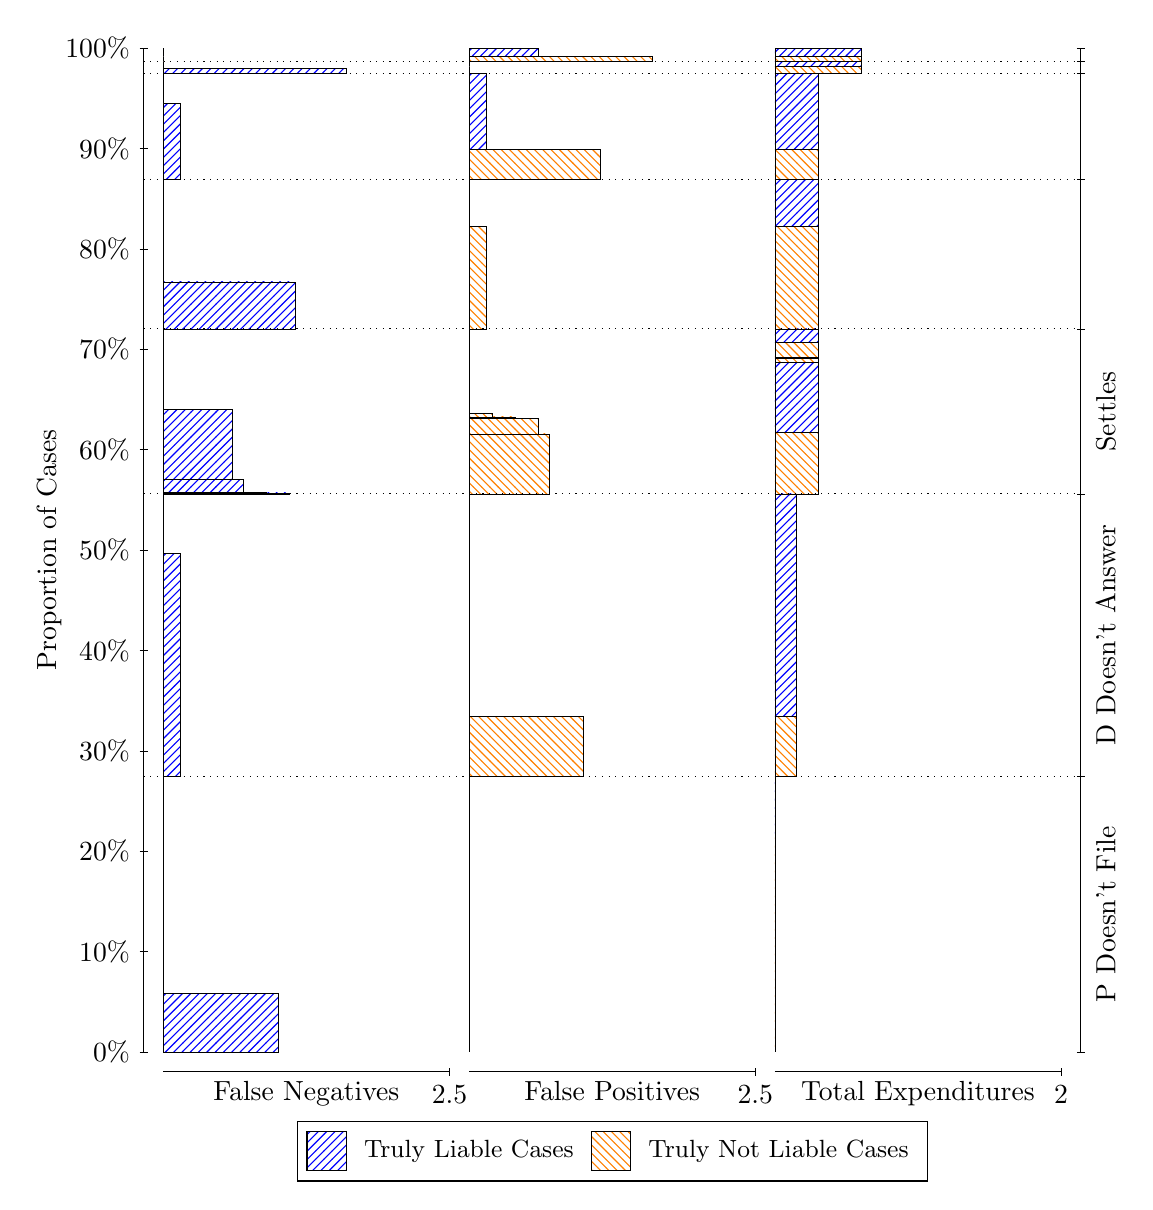
\begin{tikzpicture}
\draw[black, very thin] (1.5,1.75) -- (1.5,14.5);
\node[rotate=90, text=black, anchor=center] at (0.3, 8.125) {Proportion of Cases};
\draw[black, very thin] (1.45,1.75) -- (1.55,1.75);
\node[text=black, anchor=east] at (1.45, 1.75) {0\%};
\draw[black, very thin] (1.45,3.025) -- (1.55,3.025);
\node[text=black, anchor=east] at (1.45, 3.025) {10\%};
\draw[black, very thin] (1.45,4.3) -- (1.55,4.3);
\node[text=black, anchor=east] at (1.45, 4.3) {20\%};
\draw[black, very thin] (1.45,5.575) -- (1.55,5.575);
\node[text=black, anchor=east] at (1.45, 5.575) {30\%};
\draw[black, very thin] (1.45,6.85) -- (1.55,6.85);
\node[text=black, anchor=east] at (1.45, 6.85) {40\%};
\draw[black, very thin] (1.45,8.125) -- (1.55,8.125);
\node[text=black, anchor=east] at (1.45, 8.125) {50\%};
\draw[black, very thin] (1.45,9.4) -- (1.55,9.4);
\node[text=black, anchor=east] at (1.45, 9.4) {60\%};
\draw[black, very thin] (1.45,10.675) -- (1.55,10.675);
\node[text=black, anchor=east] at (1.45, 10.675) {70\%};
\draw[black, very thin] (1.45,11.95) -- (1.55,11.95);
\node[text=black, anchor=east] at (1.45, 11.95) {80\%};
\draw[black, very thin] (1.45,13.225) -- (1.55,13.225);
\node[text=black, anchor=east] at (1.45, 13.225) {90\%};
\draw[black, very thin] (1.45,14.5) -- (1.55,14.5);
\node[text=black, anchor=east] at (1.45, 14.5) {100\%};

\draw[black, very thin] (13.4,1.75) -- (13.4,14.5);
\draw[black, very thin] (13.35,1.75) -- (13.45,1.75);
\node[anchor=west] at (13.35, 1.75) {};
\draw[black, very thin] (13.35,5.2508) -- (13.45,5.2508);
\node[anchor=west] at (13.35, 5.2508) {};
\draw[black, very thin] (13.35,8.8384) -- (13.45,8.8384);
\node[anchor=west] at (13.35, 8.8384) {};
\draw[black, very thin] (13.35,10.934) -- (13.45,10.934);
\node[anchor=west] at (13.35, 10.934) {};
\draw[black, very thin] (13.35,12.831) -- (13.45,12.831);
\node[anchor=west] at (13.35, 12.831) {};
\draw[black, very thin] (13.35,14.18) -- (13.45,14.18);
\node[anchor=west] at (13.35, 14.18) {};
\draw[black, very thin] (13.35,14.328) -- (13.45,14.328);
\node[anchor=west] at (13.35, 14.328) {};
\draw[black, very thin] (13.35,14.5) -- (13.45,14.5);
\node[anchor=west] at (13.35, 14.5) {};

\draw[black, very thin, pattern color=blue, pattern=north east lines] (1.75,1.75) rectangle (3.2033,2.4941);
\draw[black, very thin, pattern color=orange, pattern=north west lines] (1.75,2.4941) rectangle (1.75,5.2508);
\draw[black, very thin, pattern color=blue, pattern=north east lines] (1.75,5.2508) rectangle (1.968,8.0804);
\draw[black, very thin, pattern color=orange, pattern=north west lines] (1.75,8.0804) rectangle (1.75,8.8384);
\draw[black, very thin, pattern color=blue, pattern=north east lines] (1.75,8.8384) rectangle (3.3487,8.85);
\draw[black, very thin, pattern color=blue, pattern=north east lines] (1.75,8.85) rectangle (3.058,8.8592);
\draw[black, very thin, pattern color=blue, pattern=north east lines] (1.75,8.8592) rectangle (2.7673,9.0266);
\draw[black, very thin, pattern color=blue, pattern=north east lines] (1.75,9.0266) rectangle (2.622,9.9092);
\draw[black, very thin, pattern color=orange, pattern=north west lines] (1.75,9.9092) rectangle (1.75,10.934);
\draw[black, very thin, pattern color=blue, pattern=north east lines] (1.75,10.934) rectangle (3.4213,11.53);
\draw[black, very thin, pattern color=orange, pattern=north west lines] (1.75,11.53) rectangle (1.75,12.831);
\draw[black, very thin, pattern color=blue, pattern=north east lines] (1.75,12.831) rectangle (1.968,13.797);
\draw[black, very thin, pattern color=orange, pattern=north west lines] (1.75,13.797) rectangle (1.75,14.18);
\draw[black, very thin, pattern color=blue, pattern=north east lines] (1.75,14.18) rectangle (4.0753,14.243);
\draw[black, very thin, pattern color=orange, pattern=north west lines] (1.75,14.243) rectangle (1.75,14.328);
\draw[black, very thin, pattern color=orange, pattern=north west lines] (1.75,14.328) rectangle (1.75,14.395);
\draw[black, very thin, pattern color=blue, pattern=north east lines] (1.75,14.395) rectangle (1.75,14.5);
\draw[black, very thin, pattern color=orange, pattern=north west lines] (5.6333,1.75) rectangle (5.6333,4.5067);
\draw[black, very thin, pattern color=blue, pattern=north east lines] (5.6333,4.5067) rectangle (5.6333,5.2508);
\draw[black, very thin, pattern color=orange, pattern=north west lines] (5.6333,5.2508) rectangle (7.0867,6.0088);
\draw[black, very thin, pattern color=blue, pattern=north east lines] (5.6333,6.0088) rectangle (5.6333,8.8384);
\draw[black, very thin, pattern color=orange, pattern=north west lines] (5.6333,8.8384) rectangle (6.6507,9.5993);
\draw[black, very thin, pattern color=orange, pattern=north west lines] (5.6333,9.5993) rectangle (6.5053,9.7978);
\draw[black, very thin, pattern color=orange, pattern=north west lines] (5.6333,9.7978) rectangle (6.2147,9.8162);
\draw[black, very thin, pattern color=orange, pattern=north west lines] (5.6333,9.8162) rectangle (5.924,9.8628);
\draw[black, very thin, pattern color=blue, pattern=north east lines] (5.6333,9.8628) rectangle (5.6333,10.934);
\draw[black, very thin, pattern color=orange, pattern=north west lines] (5.6333,10.934) rectangle (5.8513,12.235);
\draw[black, very thin, pattern color=blue, pattern=north east lines] (5.6333,12.235) rectangle (5.6333,12.831);
\draw[black, very thin, pattern color=orange, pattern=north west lines] (5.6333,12.831) rectangle (7.3047,13.214);
\draw[black, very thin, pattern color=blue, pattern=north east lines] (5.6333,13.214) rectangle (5.8513,14.18);
\draw[black, very thin, pattern color=orange, pattern=north west lines] (5.6333,14.18) rectangle (5.6333,14.265);
\draw[black, very thin, pattern color=blue, pattern=north east lines] (5.6333,14.265) rectangle (5.6333,14.328);
\draw[black, very thin, pattern color=orange, pattern=north west lines] (5.6333,14.328) rectangle (7.9587,14.395);
\draw[black, very thin, pattern color=blue, pattern=north east lines] (5.6333,14.395) rectangle (6.5053,14.5);
\draw[black, very thin, pattern color=orange, pattern=north west lines] (9.5167,1.75) rectangle (9.5167,4.5067);
\draw[black, very thin, pattern color=blue, pattern=north east lines] (9.5167,4.5067) rectangle (9.5167,5.2508);
\draw[black, very thin, pattern color=orange, pattern=north west lines] (9.5167,5.2508) rectangle (9.7892,6.0088);
\draw[black, very thin, pattern color=blue, pattern=north east lines] (9.5167,6.0088) rectangle (9.7892,8.8384);
\draw[black, very thin, pattern color=orange, pattern=north west lines] (9.5167,8.8384) rectangle (10.062,9.6178);
\draw[black, very thin, pattern color=blue, pattern=north east lines] (9.5167,9.6178) rectangle (10.062,10.51);
\draw[black, very thin, pattern color=orange, pattern=north west lines] (9.5167,10.51) rectangle (10.062,10.556);
\draw[black, very thin, pattern color=blue, pattern=north east lines] (9.5167,10.556) rectangle (10.062,10.568);
\draw[black, very thin, pattern color=orange, pattern=north west lines] (9.5167,10.568) rectangle (10.062,10.766);
\draw[black, very thin, pattern color=blue, pattern=north east lines] (9.5167,10.766) rectangle (10.062,10.934);
\draw[black, very thin, pattern color=orange, pattern=north west lines] (9.5167,10.934) rectangle (10.062,12.235);
\draw[black, very thin, pattern color=blue, pattern=north east lines] (9.5167,12.235) rectangle (10.062,12.831);
\draw[black, very thin, pattern color=orange, pattern=north west lines] (9.5167,12.831) rectangle (10.062,13.214);
\draw[black, very thin, pattern color=blue, pattern=north east lines] (9.5167,13.214) rectangle (10.062,14.18);
\draw[black, very thin, pattern color=orange, pattern=north west lines] (9.5167,14.18) rectangle (10.607,14.265);
\draw[black, very thin, pattern color=blue, pattern=north east lines] (9.5167,14.265) rectangle (10.607,14.328);
\draw[black, very thin, pattern color=orange, pattern=north west lines] (9.5167,14.328) rectangle (10.607,14.395);
\draw[black, very thin, pattern color=blue, pattern=north east lines] (9.5167,14.395) rectangle (10.607,14.5);
\draw[black, dotted] (1.5,5.2508) -- (13.4,5.2508);
\draw[black, dotted] (1.5,8.8384) -- (13.4,8.8384);
\draw[black, dotted] (1.5,10.934) -- (13.4,10.934);
\draw[black, dotted] (1.5,12.831) -- (13.4,12.831);
\draw[black, dotted] (1.5,14.18) -- (13.4,14.18);
\draw[black, dotted] (1.5,14.328) -- (13.4,14.328);
\draw[black, very thin] (1.75,1.5) -- (5.3833,1.5);
\node[text=black, anchor=north] at (3.5667, 1.5) {False Negatives};
\draw[black, very thin] (5.3833,1.45) -- (5.3833,1.55);
\node[text=black, anchor=north] at (5.3833, 1.45) {2.5};

\draw[black, very thin] (5.6333,1.5) -- (9.2667,1.5);
\node[text=black, anchor=north] at (7.45, 1.5) {False Positives};
\draw[black, very thin] (9.2667,1.45) -- (9.2667,1.55);
\node[text=black, anchor=north] at (9.2667, 1.45) {2.5};

\draw[black, very thin] (9.5167,1.5) -- (13.15,1.5);
\node[text=black, anchor=north] at (11.333, 1.5) {Total Expenditures};
\draw[black, very thin] (13.15,1.45) -- (13.15,1.55);
\node[text=black, anchor=north] at (13.15, 1.45) {2};

\node[text=black, centered, rotate=90] at (13.72, 3.5004) {\contour{white}{P Doesn't File}};
\node[text=black, centered, rotate=90] at (13.72, 7.0446) {\contour{white}{D Doesn't Answer}};
\node[text=black, centered, rotate=90] at (13.72, 9.886) {\contour{white}{Settles}};





\draw (7.449999999999999,1.5) node[draw=none] (baseCoordinate) {};
\begin{scope}[align=center]
        \matrix[scale=0.5, draw=black, below=0.5cm of baseCoordinate, nodes={draw}, column sep=0.1cm]{
            \node[rectangle, draw, minimum width=0.5cm, minimum height=0.5cm, pattern color=blue, pattern=north east lines] {}; &
            \node[draw=none, font=\small, text=black] (B) {Truly Liable Cases}; &
            \node[rectangle, draw, minimum width=0.5cm, minimum height=0.5cm, pattern color=orange, pattern=north west lines] {}; &
            \node[draw=none, font=\small, text=black] (B) {Truly Not Liable Cases}; \\
            };
\end{scope}

\end{tikzpicture}
\end{document}